\documentclass{ximera}

%\usepackage{todonotes}
%\usepackage{mathtools} %% Required for wide table Curl and Greens
%\usepackage{cuted} %% Required for wide table Curl and Greens
\newcommand{\todo}{}

\usepackage{esint} % for \oiint
\ifxake%%https://math.meta.stackexchange.com/questions/9973/how-do-you-render-a-closed-surface-double-integral
\renewcommand{\oiint}{{\large\bigcirc}\kern-1.56em\iint}
\fi


\graphicspath{
  {./}
  {ximeraTutorial/}
  {basicPhilosophy/}
  {functionsOfSeveralVariables/}
  {normalVectors/}
  {lagrangeMultipliers/}
  {vectorFields/}
  {greensTheorem/}
  {shapeOfThingsToCome/}
  {dotProducts/}
  {partialDerivativesAndTheGradientVector/}
  {../productAndQuotientRules/exercises/}
  {../normalVectors/exercisesParametricPlots/}
  {../continuityOfFunctionsOfSeveralVariables/exercises/}
  {../partialDerivativesAndTheGradientVector/exercises/}
  {../directionalDerivativeAndChainRule/exercises/}
  {../commonCoordinates/exercisesCylindricalCoordinates/}
  {../commonCoordinates/exercisesSphericalCoordinates/}
  {../greensTheorem/exercisesCurlAndLineIntegrals/}
  {../greensTheorem/exercisesDivergenceAndLineIntegrals/}
  {../shapeOfThingsToCome/exercisesDivergenceTheorem/}
  {../greensTheorem/}
  {../shapeOfThingsToCome/}
  {../separableDifferentialEquations/exercises/}
  {vectorFields/}
}

\newcommand{\mooculus}{\textsf{\textbf{MOOC}\textnormal{\textsf{ULUS}}}}

\usepackage{tkz-euclide}\usepackage{tikz}
\usepackage{tikz-cd}
\usetikzlibrary{arrows}
\tikzset{>=stealth,commutative diagrams/.cd,
  arrow style=tikz,diagrams={>=stealth}} %% cool arrow head
\tikzset{shorten <>/.style={ shorten >=#1, shorten <=#1 } } %% allows shorter vectors

\usetikzlibrary{backgrounds} %% for boxes around graphs
\usetikzlibrary{shapes,positioning}  %% Clouds and stars
\usetikzlibrary{matrix} %% for matrix
\usepgfplotslibrary{polar} %% for polar plots
\usepgfplotslibrary{fillbetween} %% to shade area between curves in TikZ
\usetkzobj{all}
\usepackage[makeroom]{cancel} %% for strike outs
%\usepackage{mathtools} %% for pretty underbrace % Breaks Ximera
%\usepackage{multicol}
\usepackage{pgffor} %% required for integral for loops



%% http://tex.stackexchange.com/questions/66490/drawing-a-tikz-arc-specifying-the-center
%% Draws beach ball
\tikzset{pics/carc/.style args={#1:#2:#3}{code={\draw[pic actions] (#1:#3) arc(#1:#2:#3);}}}



\usepackage{array}
\setlength{\extrarowheight}{+.1cm}
\newdimen\digitwidth
\settowidth\digitwidth{9}
\def\divrule#1#2{
\noalign{\moveright#1\digitwidth
\vbox{\hrule width#2\digitwidth}}}





\newcommand{\RR}{\mathbb R}
\newcommand{\R}{\mathbb R}
\newcommand{\N}{\mathbb N}
\newcommand{\Z}{\mathbb Z}

\newcommand{\sagemath}{\textsf{SageMath}}


%\renewcommand{\d}{\,d\!}
\renewcommand{\d}{\mathop{}\!d}
\newcommand{\dd}[2][]{\frac{\d #1}{\d #2}}
\newcommand{\pp}[2][]{\frac{\partial #1}{\partial #2}}
\renewcommand{\l}{\ell}
\newcommand{\ddx}{\frac{d}{\d x}}

\newcommand{\zeroOverZero}{\ensuremath{\boldsymbol{\tfrac{0}{0}}}}
\newcommand{\inftyOverInfty}{\ensuremath{\boldsymbol{\tfrac{\infty}{\infty}}}}
\newcommand{\zeroOverInfty}{\ensuremath{\boldsymbol{\tfrac{0}{\infty}}}}
\newcommand{\zeroTimesInfty}{\ensuremath{\small\boldsymbol{0\cdot \infty}}}
\newcommand{\inftyMinusInfty}{\ensuremath{\small\boldsymbol{\infty - \infty}}}
\newcommand{\oneToInfty}{\ensuremath{\boldsymbol{1^\infty}}}
\newcommand{\zeroToZero}{\ensuremath{\boldsymbol{0^0}}}
\newcommand{\inftyToZero}{\ensuremath{\boldsymbol{\infty^0}}}



\newcommand{\numOverZero}{\ensuremath{\boldsymbol{\tfrac{\#}{0}}}}
\newcommand{\dfn}{\textbf}
%\newcommand{\unit}{\,\mathrm}
\newcommand{\unit}{\mathop{}\!\mathrm}
\newcommand{\eval}[1]{\bigg[ #1 \bigg]}
\newcommand{\seq}[1]{\left( #1 \right)}
\renewcommand{\epsilon}{\varepsilon}
\renewcommand{\phi}{\varphi}


\renewcommand{\iff}{\Leftrightarrow}

\DeclareMathOperator{\arccot}{arccot}
\DeclareMathOperator{\arcsec}{arcsec}
\DeclareMathOperator{\arccsc}{arccsc}
\DeclareMathOperator{\si}{Si}
\DeclareMathOperator{\scal}{scal}
\DeclareMathOperator{\sign}{sign}


%% \newcommand{\tightoverset}[2]{% for arrow vec
%%   \mathop{#2}\limits^{\vbox to -.5ex{\kern-0.75ex\hbox{$#1$}\vss}}}
\newcommand{\arrowvec}[1]{{\overset{\rightharpoonup}{#1}}}
%\renewcommand{\vec}[1]{\arrowvec{\mathbf{#1}}}
\renewcommand{\vec}[1]{{\overset{\boldsymbol{\rightharpoonup}}{\mathbf{#1}}}\hspace{0in}}

\newcommand{\point}[1]{\left(#1\right)} %this allows \vector{ to be changed to \vector{ with a quick find and replace
\newcommand{\pt}[1]{\mathbf{#1}} %this allows \vec{ to be changed to \vec{ with a quick find and replace
\newcommand{\Lim}[2]{\lim_{\point{#1} \to \point{#2}}} %Bart, I changed this to point since I want to use it.  It runs through both of the exercise and exerciseE files in limits section, which is why it was in each document to start with.

\DeclareMathOperator{\proj}{\mathbf{proj}}
\newcommand{\veci}{{\boldsymbol{\hat{\imath}}}}
\newcommand{\vecj}{{\boldsymbol{\hat{\jmath}}}}
\newcommand{\veck}{{\boldsymbol{\hat{k}}}}
\newcommand{\vecl}{\vec{\boldsymbol{\l}}}
\newcommand{\uvec}[1]{\mathbf{\hat{#1}}}
\newcommand{\utan}{\mathbf{\hat{t}}}
\newcommand{\unormal}{\mathbf{\hat{n}}}
\newcommand{\ubinormal}{\mathbf{\hat{b}}}

\newcommand{\dotp}{\bullet}
\newcommand{\cross}{\boldsymbol\times}
\newcommand{\grad}{\boldsymbol\nabla}
\newcommand{\divergence}{\grad\dotp}
\newcommand{\curl}{\grad\cross}
%\DeclareMathOperator{\divergence}{divergence}
%\DeclareMathOperator{\curl}[1]{\grad\cross #1}
\newcommand{\lto}{\mathop{\longrightarrow\,}\limits}

\renewcommand{\bar}{\overline}

\colorlet{textColor}{black}
\colorlet{background}{white}
\colorlet{penColor}{blue!50!black} % Color of a curve in a plot
\colorlet{penColor2}{red!50!black}% Color of a curve in a plot
\colorlet{penColor3}{red!50!blue} % Color of a curve in a plot
\colorlet{penColor4}{green!50!black} % Color of a curve in a plot
\colorlet{penColor5}{orange!80!black} % Color of a curve in a plot
\colorlet{penColor6}{yellow!70!black} % Color of a curve in a plot
\colorlet{fill1}{penColor!20} % Color of fill in a plot
\colorlet{fill2}{penColor2!20} % Color of fill in a plot
\colorlet{fillp}{fill1} % Color of positive area
\colorlet{filln}{penColor2!20} % Color of negative area
\colorlet{fill3}{penColor3!20} % Fill
\colorlet{fill4}{penColor4!20} % Fill
\colorlet{fill5}{penColor5!20} % Fill
\colorlet{gridColor}{gray!50} % Color of grid in a plot

\newcommand{\surfaceColor}{violet}
\newcommand{\surfaceColorTwo}{redyellow}
\newcommand{\sliceColor}{greenyellow}




\pgfmathdeclarefunction{gauss}{2}{% gives gaussian
  \pgfmathparse{1/(#2*sqrt(2*pi))*exp(-((x-#1)^2)/(2*#2^2))}%
}


%%%%%%%%%%%%%
%% Vectors
%%%%%%%%%%%%%

%% Simple horiz vectors
\renewcommand{\vector}[1]{\left\langle #1\right\rangle}


%% %% Complex Horiz Vectors with angle brackets
%% \makeatletter
%% \renewcommand{\vector}[2][ , ]{\left\langle%
%%   \def\nextitem{\def\nextitem{#1}}%
%%   \@for \el:=#2\do{\nextitem\el}\right\rangle%
%% }
%% \makeatother

%% %% Vertical Vectors
%% \def\vector#1{\begin{bmatrix}\vecListA#1,,\end{bmatrix}}
%% \def\vecListA#1,{\if,#1,\else #1\cr \expandafter \vecListA \fi}

%%%%%%%%%%%%%
%% End of vectors
%%%%%%%%%%%%%

%\newcommand{\fullwidth}{}
%\newcommand{\normalwidth}{}



%% makes a snazzy t-chart for evaluating functions
%\newenvironment{tchart}{\rowcolors{2}{}{background!90!textColor}\array}{\endarray}

%%This is to help with formatting on future title pages.
\newenvironment{sectionOutcomes}{}{}



%% Flowchart stuff
%\tikzstyle{startstop} = [rectangle, rounded corners, minimum width=3cm, minimum height=1cm,text centered, draw=black]
%\tikzstyle{question} = [rectangle, minimum width=3cm, minimum height=1cm, text centered, draw=black]
%\tikzstyle{decision} = [trapezium, trapezium left angle=70, trapezium right angle=110, minimum width=3cm, minimum height=1cm, text centered, draw=black]
%\tikzstyle{question} = [rectangle, rounded corners, minimum width=3cm, minimum height=1cm,text centered, draw=black]
%\tikzstyle{process} = [rectangle, minimum width=3cm, minimum height=1cm, text centered, draw=black]
%\tikzstyle{decision} = [trapezium, trapezium left angle=70, trapezium right angle=110, minimum width=3cm, minimum height=1cm, text centered, draw=black]

\author{Bart Snapp \and Jim Talamo}

\outcome{Represent a function of several variables graphically and by using contour plots.}
\outcome{Introduce the idea of curves on surfaces corresponding to a curve in the domain.}
\outcome{Introduce level curves as special examples of curves in the domain of the function.}

\title[Dig-In:]{Level sets}

\begin{document}
\begin{abstract}
  We introduce level sets.
\end{abstract}
\maketitle




\section{Level sets}

It was Descartes who said ``\link[Je pense, donc je
  suis]{https://en.wikipedia.org/wiki/Cogito,_ergo_sum}.'' He also
developed our rectangular coordinate system, the $(x,y)$-plane. This
is also known as the \link[Cartesian coordinate
  system]{https://en.wikipedia.org/wiki/Cartesian_coordinate_system}.
This coordinate system allows us to consider the graph of a
function. First, recall that the graph of a function of a single
variable, $y=f(x)$ is a curve in a two-dimensional plane.  In the same
sense, the graph of a function of two variables, $z = F(x,y)$ is a
surface in three-dimensional space. The graph of a function of three
variables, $w=F(x,y,z)$ is a surface in \textit{four}-dimensional
space. A surface in higher than three dimensions is often called a
\dfn{hypersurface}. How can we visualize such functions?  For
visualizing functions $f:\R\to\R$, a graphing utility like
\link[\textsl{Desmos}]{https://www.desmos.com/} is really great. For
visualizing functions $F:\R^2\to\R$,
\link[\textsl{GeoGebra}]{https://www.geogebra.org/3d} is very
helpful. However, once we get to functions $F:\R^3\to\R$ (or $F: \R^n \to \R$), visualizing 
the graph of the function as we do in two and three dimensions 
becomes much more difficult.  One
powerful technique to help us understand a function $F:\R^3\to\R$
visually is known as sketching \textit{level sets}.


\begin{definition}
  Suppose that $F:\R^n \to \R$ is a function and $c$ is in the range
  of $F$. A \dfn{level set} corresponding to $F(\vec{x})=c$ is a set
  in the domain of the function such that $F(\vec{x}) = c$ for all
  points in the set.
\end{definition}

When working with functions $F:\R^2\to\R$ the level sets are known as
\dfn{level curves}.

When we are looking at level curves, we can think about choosing
a $z$-value, say $z=c$, in the range of the function and ask ``at
which points $(x,y)$ can we evaluate the function to get $F(x,y)=c$?''
Those points form our level curve.    If we choose a value $z=c$ 
that was not in the range of $F$, there would be no points in the 
$(x,y)$-plane for which $F(x,y)=c$, and hence no level curve 
associated to $z = c$.

%% \begin{remark}
%% Some people call the curve on the surface $z=F(x,y)$ that lies
%% directly above (or below) the level curve a \dfn{contour curve}.
%% \end{remark}


It may be surprising to find that the concept of level sets is
familiar to most people, but they don't realize it.  Topographical
maps, like the one below represent the surface of Earth by
indicating points with the same elevation with \dfn{contour
  lines}.  We also had an example of the contour lines of Meteor 
  Crater as we began this section.

\begin{image}%%Allegheny College: http://sitesmedia.s3.amazonaws.com/creekconnections/files/2014/09/topomap.jpg
  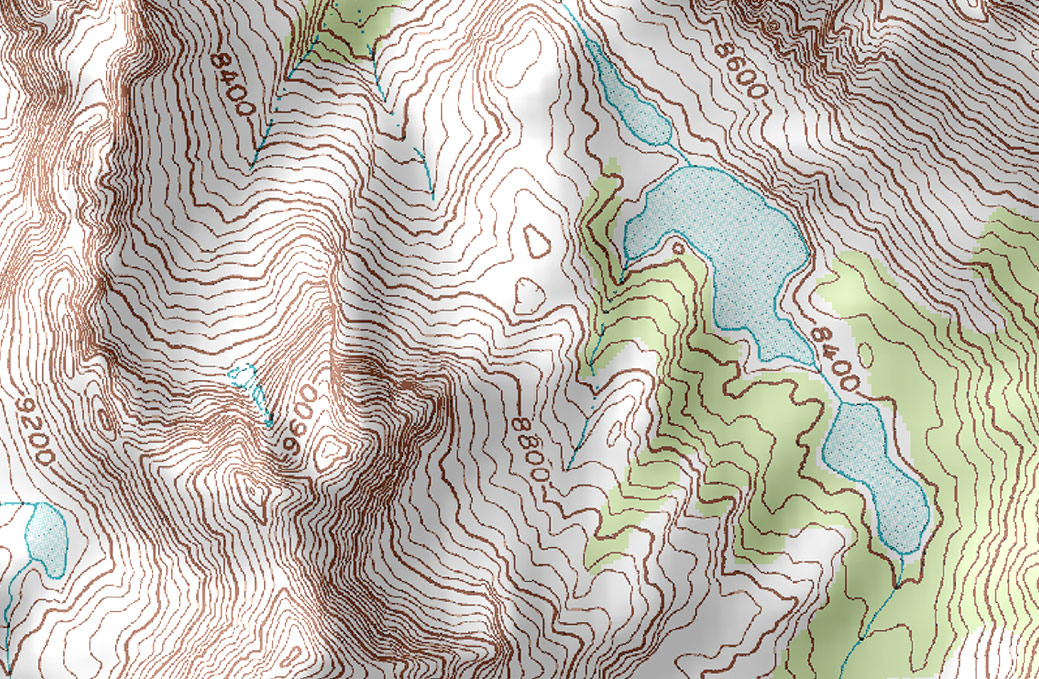
\includegraphics{topomap.jpg}
\end{image}

Another example you may know are \dfn{isotherms}, which are curves along which the
temperature does not change. We see these in weather maps.

\begin{image}
  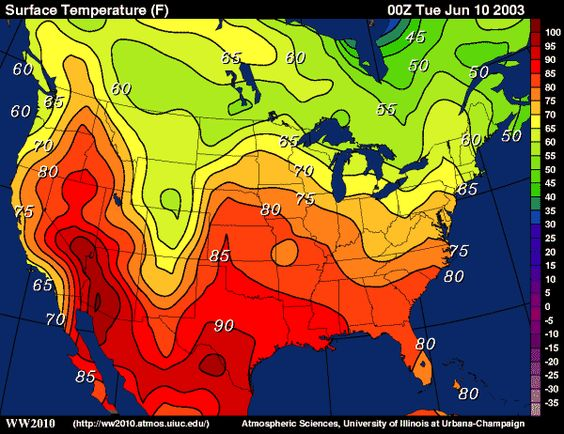
\includegraphics{isotherm.jpg}
\end{image}

 Below we see a surface with level curves drawn
beneath the surface.  Remember that the level curves are in the 
domain of the function, not on the surface itself.

\begin{image}
  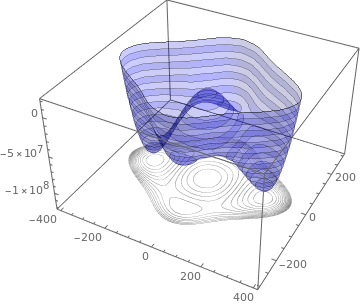
\includegraphics{firstContourPlot.png}
\end{image}


\begin{example}
  Given that $z=c$ is in the range of $z=F(x,y)$, select the
  statements below that are true.
  \begin{selectAll}
    \choice[correct]{The level curves $F(x,y)=c$ are in the domain of the function.} 
    \choice[correct]{The level curves $F(x,y)=c$ are in the $(x,y)$-plane.} 
    \choice{The level curves $F(x,y)=c$ are in the range of the function.} 
    \choice{The level curves $F(x,y)=c$ are on the surface $z=F(x,y)$.} 
    \choice{The level curves $F(x,y)=c$ can also be thought of as the intersection of the plane $z=c$ with the surface $z=F(x,y)$.} 
  \end{selectAll}
\end{example}


We often mark the function value on the corresponding level set. 
If we choose function values which have a constant difference, then level
curves are close together when the function values are changing rapidly, and
far apart when the function values are changing slowly.

\begin{question}
  Suppose you have a differentiable function $F:\R^2\to\R$ with the following set of
  level curves.  You should interpolate reasonable values of the function $F$  
  between the level curves which are shown:
  \begin{image}
    \begin{tikzpicture}	
      \draw[ultra thick, penColor] (0,0) ellipse (1.1cm and .8cm);
      \draw[ultra thick, penColor] (.3,0) ellipse (1.5cm and 1cm);
      \draw[ultra thick, penColor] (.7,0) ellipse (2cm and 1.2cm);
      \draw[ultra thick, penColor] (1,0) ellipse (2.4cm and 1.5cm);
      \draw[ultra thick, penColor] (1.3,0) ellipse (2.8cm and 1.8cm);
      \draw[ultra thick, penColor] (1.6,0) ellipse (3.2cm and 2.1cm);

      \node[penColor,fill=white] at (.6,-.6) {\small$7$};
      \node[penColor,fill=white] at (1.2,-.8) {\small$6$};
      \node[penColor,fill=white] at (1.8,-1) {\small$5$};
      \node[penColor,fill=white] at (2.4,-1.2) {\small$4$};
      \node[penColor,fill=white] at (3,-1.4) {\small$3$};
      \node[penColor,fill=white] at (3.6,-1.6) {\small$2$};

      \draw[fill=black,black] (3.7,0) circle (.1cm);
      \draw[fill=black,black] (1.3,1.65) circle (.1cm);
      \draw[fill=black,black] (-1.3,0) circle (.1cm);

      \node[black] at (-2,0) {$B$};
      \node[black] at (.8,2.5) {$A$};
      \node[black,above] at (3.7,0) {$C$};

      \draw[thick,->] (-1.8,0) -- (-1.5,0);
      \draw[thick,->] (.9,2.3) -- (1.2,1.7);
    \end{tikzpicture}
  \end{image}
  Consider the points $A$, $B$, and $C$ on the surface
  $z=F(x,y)$. Order the points from least steep to most steep.


  \begin{prompt}
    At point $\answer[format=string]{C}$ the surface is less steep
    than at point $\answer[format=string]{A}$, and the surface is
    steepest at point $\answer[format=string]{B}$.
    \begin{feedback}
    Since the $z$-values on the level curves are equally spaced in this 
    example, level curves which are close together indicate more rapid 
    change in the $z$-values, while level curves which are further apart 
    indicate slower change in the $z$-values.
    \end{feedback}
  \end{prompt}
\end{question}

Now, let's see if you can identify some simple surfaces based on their level curves.

\begin{question}
  Match the following level surfaces to the equations below.
  \begin{center}
    \resizebox{1in}{!}{
    \begin{tikzpicture}
      \node[gray] at (2.5,2.5) {\Huge\textbf{A}};
      \draw[ultra thick, penColor] (0,0) -- (5,0) -- (5,5) -- (0,5) -- (0,0);
      \draw[thick, penColor] (3,0) -- (5,2);
      \draw[thick, penColor] (1,0) -- (5,4);
      \draw[thick, penColor] (0,1) -- (4,5);
      \draw[thick, penColor] (0,3) -- (2,5);
    \end{tikzpicture}}
    \quad
    \resizebox{1in}{!}{
    \begin{tikzpicture}
      \node[gray] at (2.5,2.5) {\Huge\textbf{B}};
      \draw[ultra thick, penColor] (0,0) -- (5,0) -- (5,5) -- (0,5) -- (0,0);
      \draw[thick, penColor] (2,0) -- (0,2);
      \draw[thick, penColor] (4,0) -- (0,4);
      \draw[thick, penColor] (5,1) -- (1,5);
      \draw[thick, penColor] (5,3) -- (3,5);
    \end{tikzpicture}}
  \end{center}
  \begin{center}
    \resizebox{1in}{!}{
      \begin{tikzpicture}
      \node[gray] at (2.5,2.5) {\Huge\textbf{C}};
      \draw[ultra thick, penColor] (0,0) -- (5,0) -- (5,5) -- (0,5) -- (0,0);
      \draw[thick, penColor] (0,1) -- (5,1);
      \draw[thick, penColor] (0,2) -- (5,2);
      \draw[thick, penColor] (0,3) -- (5,3);
      \draw[thick, penColor] (0,4) -- (5,4);
    \end{tikzpicture}}
    \quad
    \resizebox{1in}{!}{
      \begin{tikzpicture}
      \node[gray] at (2.5,2.5) {\Huge\textbf{D}};
      \draw[ultra thick, penColor] (0,0) -- (5,0) -- (5,5) -- (0,5) -- (0,0);
      \draw[thick, penColor] (1,0) -- (1,5);
      \draw[thick, penColor] (2,0) -- (2,5);
      \draw[thick, penColor] (3,0) -- (3,5);
      \draw[thick, penColor] (4,0) -- (4,5);
    \end{tikzpicture}}
  \end{center}
  \begin{align*}
    &\answer[format=string]{D}: x+z=3\\
    &\answer[format=string]{C}: y+z=-2\\
    &\answer[format=string]{B}: x+y+z=-3\\
    &\answer[format=string]{A}: -x+y+z=2
  \end{align*}
\end{question}




%\subsection{Working with level curves}

%Let's work within the scenario for functions $F:\R^2 \to \R$ since
%they are easier to visualize.  The idea behind a level set is fairly
%intuitive.  Rather than picking points along a grid in the
%$(x,y)$-plane and evaluating the function at these points, we can pick
%a $z$-value, say $z=c$, in the range of the function and ask ``at
%which points $(x,y)$ can we evaluate the function to get $F(x,y)=c$?''
%Those points form our level set.  Before moving on, take a second to
%try to visualize what we just described for a function $z=F(x,y)$.

Let's look at another example.



\begin{example}
  Suppose that $F(x,y) = x^2-y^2$. Sketch the level curves of $F$ for
  $c=-3$, $-2$, $-1$, $0$, $1$, $2$, and $3$.
  \begin{explanation}
    First, notice that the domain of $F$ is $\R^2$, and the range of $F$ is 
    also $\R^2$.   It's particularly important to notice that all 
    of the values of $c$ we will use to find level curves are in the range 
    of $F$.
    
      Now let's find the level curves of $F$ for the required values.
      Each of our level curves will be of the form
      \[
      c = \answer[given]{x^2-y^2}
      \]
      Now we just need to substitute all of our values for $c$ and
      plot each of the following implicit functions:
    \begin{align*}
      -3 &= x^2-y^2\\
      -2 &= x^2-y^2\\
      -1 &= x^2-y^2\\
       0 &= x^2-y^2\\
       1 &= x^2-y^2\\
       2 &= x^2-y^2\\
       3 &= x^2-y^2
    \end{align*}
     To make your sketch, either plot these implicit functions with your favorite
    graphing device, or recognize that they are crossing lines when
    $x=y=0$ and hyperbolas otherwise.
    \begin{onlineOnly}
      As a gesture of friendship, we have included a graph of these
      level curves.
      \[
      \graph[xmin=-5, xmax=5, ymin=-2.5, ymax=2.5]{-3=x^2-y^2,-2=x^2-y^2,-1=x^2-y^2,0=x^2-y^2,1=x^2-y^2,2=x^2-y^2,3=x^2-y^2}
      \]
    \end{onlineOnly}
    Below, we evaluate $F$ on our level curves and plot the resulting 
    curves on the surface $F$.
    \begin{image}
      \begin{tikzpicture}
        \begin{axis}%
          [tick label style={font=\scriptsize},axis on top,
	    axis lines=center,
	    view={147}{30},
	    name=myplot,
	    %xtick=\empty,
	    %ytick=\empty,
	    %ztick=\empty,
	    ymin=-3.5,ymax=3.5,
	    xmin=-3.5,xmax=3.5,
	    zmin=-3.5, zmax=3.5,
	    every axis x label/.style={at={(axis cs:\pgfkeysvalueof{/pgfplots/xmax},0,0)},xshift=-5pt,yshift=-1pt},
            xlabel={\scriptsize $x$},
            every axis y label/.style={at={(axis cs:0,\pgfkeysvalueof{/pgfplots/ymax},0)},xshift=4pt,yshift=-4pt},
            ylabel={\scriptsize $y$},
            every axis z label/.style={at={(axis cs:0,0,\pgfkeysvalueof{/pgfplots/zmax})},xshift=0pt,yshift=4pt},
            colormap/cool
	  ]
          \addplot3[mesh,samples y=15,domain=-2:2, y domain=-2:2,very thin,z buffer=sort,samples=30,] ({x},{y},{x^2-y^2});
          
          \addplot3 [very thick,penColor,domain=-2:2,smooth,samples=60,samples y=0] ({x},{x},0);
          \addplot3 [very thick,penColor,domain=-2:2,smooth,samples=60,samples y=0] ({x},{-x},0);
          
          \addplot3 [very thick,penColor, smooth,samples=60,samples y=0,domain=-1.33:1.33] ({cosh(x)},{sinh(x)},1);
          \addplot3 [very thick,penColor, smooth,samples=60,samples y=0,domain=-1.33:1.33] ({-cosh(x)},{sinh(x)},1);

          \addplot3 [very thick,penColor, smooth,samples=60,samples y=0,domain=-.9:.9] ({sqrt(2)*cosh(x)},{sqrt(2)*sinh(x)},2);
          \addplot3 [very thick,penColor, smooth,samples=60,samples y=0,domain=-.9:.9] ({-sqrt(2)*cosh(x)},{sqrt(2)*sinh(x)},2);

          \addplot3 [very thick,penColor, smooth,samples=60,samples y=0,domain=-.55:.55] ({sqrt(3)*cosh(x)},{sqrt(3)*sinh(x)},3);
          \addplot3 [very thick,penColor, smooth,samples=60,samples y=0,domain=-.55:.55] ({-sqrt(3)*cosh(x)},{sqrt(3)*sinh(x)},3);


          \addplot3 [very thick,penColor, smooth,samples=60,samples y=0,domain=-1.33:1.33] ({sinh(x)},{cosh(x)},-1);
          \addplot3 [very thick,penColor, smooth,samples=60,samples y=0,domain=-1.33:1.33] ({sinh x)},{-cosh(x)},-1);

          \addplot3 [very thick,penColor, smooth,samples=60,samples y=0,domain=-.9:.9] ({sqrt(2)*sinh(x)},{sqrt(2)*cosh(x)},-2);
          \addplot3 [very thick,penColor, smooth,samples=60,samples y=0,domain=-.9:.9] ({sqrt(2)*sinh(x)},{-sqrt(2)*cosh(x)},-2);

          \addplot3 [very thick,penColor, smooth,samples=60,samples y=0,domain=-.55:.55] ({sqrt(3)*sinh(x)},{sqrt(3)*cosh(x)},-3);
          \addplot3 [very thick,penColor, smooth,samples=60,samples y=0,domain=-.55:.55] ({sqrt(3)*sinh(x)},{-sqrt(3)*cosh(x)},-3);
          
        \end{axis}
      \end{tikzpicture}
    \end{image}
     Notice how the difference between consecutive $c$ values is always $1$, so 
    we can use the closeness of the level curves on the $(x,y)$-plane to determine 
    how the surface is changing. Near the level curves of $c=0$ and $c=1$ we 
    can both predict (from our sketch of just the level curves) as well as see (on our 
    graph of the curves on the surface) that $F$ indeed is growing quickly.
    
  \end{explanation}
\end{example}




 
%% We illustrate these ideas with a picture.  Consider the function,
%% $F(x,y) = 5-4x+y^2$.  Noting that the domain of this function is
%% $\R^2$ and the range is $\R$, we can choose any value for $c$ that we
%% want.
 
%% \begin{itemize}
%% \item If we choose $c=1$, the set of all points in the domain of $F$ for which $z=0$ is found easily by setting $z= 5-4x+y^2 = 1$.  This is the curve in the $(x,y)$-plane described by $4x-y^2 = 1$ or $x= \frac{1}{4}+ \frac{1}{4}y^2$.
%% \item If we choose $c=5$, the set of all points in the domain of $F$ for which $z=0$ is found easily by setting $z= 5-4x+y^2 = 4$. This is the curve in the $(x,y)$-plane described by $4x-y^2 = 0$ or $x= \frac{1}{4}y^2$.
%% \end{itemize}

%% We now plot the level curves and the contour curves on the same plot:   
   
%% \begin{image}
%%   \begin{tikzpicture}
%%     \begin{axis}[tick label style={font=\scriptsize},axis on top,
%% 	axis lines=center,
%% 	view={110}{25},
%% 	name=myplot,
%% 	xtick=\empty,
%%         ytick=\empty,
%%         ztick=\empty,
%% 	ymin=-1,ymax=1,
%% 	xmin=-.5,xmax=1,
%% 	zmin=-.5, zmax=9,
%% 	every axis x label/.style={at={(axis cs:\pgfkeysvalueof{/pgfplots/xmax},0,0)},xshift=-1pt,yshift=-4pt},
%% 	xlabel={\scriptsize $x$},
%% 	every axis y label/.style={at={(axis cs:0,\pgfkeysvalueof{/pgfplots/ymax},0)},xshift=5pt,yshift=-3pt},
%% 	ylabel={\scriptsize $y$},
%% 	every axis z label/.style={at={(axis cs:0,0,\pgfkeysvalueof{/pgfplots/zmax})},xshift=0pt,yshift=4pt},
%% 	zlabel={\scriptsize $z$},
%%         colormap/cool,
%%       ]
%% %      \addplot3[gray,domain=0:2,samples y=0,dashed] ({1*cos(45)},{1*sin(45)},x); %% line for z
%% %      \addplot3[gray,domain=0:cos(45),samples y=0,dashed] ({x},{1*sin(45)},0); %% line for x
%% %      \addplot3[gray,domain=0:cos(45),samples y=0,dashed] ({sin(45)},{x},0); %% line for y
%% \addplot3[domain=-1:2,y domain=-1:2,mesh,samples y=25,very thin,z buffer=sort,  samples=25,] (x,y,{5-4*x+y^2});   
%% \addplot3 [very thick,penColor, smooth,domain=-1:2,samples=20,samples y=0] ({(.25+.25*x^2)},{x},{1});
%% \addplot3 [very thick,penColor, dashed,domain=-1:2,samples=20,samples y=0] ({(.25+.25*x^2)},{x},{0});
%% \addplot3 [very thick,penColor2, smooth,domain=-1:2,samples=20,samples y=0] ({(.25*x^2)},{x},{4});
%% \addplot3 [very thick,penColor2, dashed,domain=-1:2,samples=20,samples y=0] ({(.25*x^2)},{x},{0});
%%        \end{axis}
%%   \end{tikzpicture}
  
%%  \end{image}
 
%% \begin{center}
%%   The dashed lines represent the level curves corresponding to $z=1$ and $z=5$.  The smooth lines on the surface represent the contour curves on the surface.  Note that the contour curve associated to $z=1$ can be found by ``lifting'' the corresponding level curve up $1$ unit, while the contour curve associated to $z=5$ can be found by ``lifting'' the corresponding level curve up $5$ units.
%% \end{center}

 
%%%%%%%%%%%%%%%%%%%%%%%%%%%%%%%%%%%%%%%%%%%%%%%%%%%% 

Let's see another example.

\begin{example}
Suppose that $F(x,y) = 4xy+3y^2+3$.  Find the equation of the level
curve that passes through $(x,y) = (1,2)$ in terms of $x$ and $y$, and
then find a parametric description for both the level curve as well as
the corresponding curve on the surface.

\begin{explanation}
First, find the equation of the level curve.  Note that the level
curve consists of all points in the $(x,y)$-plane that give the same
value for $F(x,y)$.  Since $(1,2)$ lies on this curve, and $F(1,2) =
\answer[given]{23}$, the equation of the level curve is $4xy+3y^2+3 =
\answer[given]{23}$, or $4xy+3y^2 = \answer[given]{20}$.


Now, we find a vector-valued function for the level curve, as well as
the curve on the surface.  Since the level curve is given by the
equation $4xy+3y^2 = 20$ and we can solve for $x$ without too much
algebra, we set $y=t$.  Then, $x =\answer[given]{\frac{20-3t^2}{4t}}$.
The level curve can be described parametrically by:
\[
\vec{p} (t) = \vector{\answer[given]{\frac{20-3t^2}{4t}}, \answer[given]{t}}
\]
The corresponding curve on the surface can be described
parametrically by:

\begin{align*}
  \vec{r} (t) &= \vector{\answer[given]{(20 - 3 t^2)/(4 t)},\answer[given]{t},F\left(\vec{p}(t) \right)} \\
  &= \vector{\answer[given]{\frac{20-3t^2}{4t}}, \answer[given]{t}, \answer[given]{23}}
\end{align*}

Notice that the $z$-component of the curve on the surface should not
require much calculation since we found the curve on the surface by
noting $F(1,2) =23$.  This means that all of the $z$-values on the
curve on the surface should be $\answer[given]{23}$.
\end{explanation}
\end{example}
  
So far, the level sets we've been working with have been curves in
$\R^2$. We can easily generalize to functions $F:\R^n \to \R$.  When
working with functions $F:\R^3\to\R$, our level sets are also called
\textit{level surfaces}.  \index{level sets}



%%%@BART: For the second example, I think you had mentioned something about quadric surfaces.  I've commented out what is below this for you to typeset such an example.%%%%%

%If one example is good, two is better.
%
%\begin{example}
%  Let $F(x,y) = \frac{x+y}{x^2+y^2+1}$. Find the level curves for $z=c$.
%  \begin{explanation}
%    We begin by setting $F(x,y)=c$ for an arbitrary $c$ and seeing if
%    algebraic manipulation of the equation reveals anything
%    significant.
%    \begin{align*}
%      \frac{x+y}{x^2+y^2+1} &= c \\
%      x+y &= \answer[given]{c(x^2+y^2+1)}.
%    \end{align*}
%    You may recognize this as a circle; regardless, plotting
%    \[
%    x+y = c(x^2+y^2+1).
%    \]
%    for $c=0,\pm 0.2$, $\pm 0.4$, and $\pm 0.6$ will reveal the shape of the
%    surface defined by $F$.
%    \begin{onlineOnly}
%      As a gesture of friendship, we have included a graph of these
%      level curves:
%      \[
%      \graph[xmin=-15, xmax=15, ymin=-7, ymax=7]{x+y = 0.6(x^2+y^2+1),x+y = 0.4(x^2+y^2+1), x+y = 0.2(x^2+y^2+1),x+y = 0,x+y = -0.2(x^2+y^2+1),x+y = -0.4(x^2+y^2+1),x+y = -0.6(x^2+y^2+1)}
%      \]
%    \end{onlineOnly}
%    \begin{image}
%      \begin{tikzpicture}
%        \begin{axis}%
%          [tick label style={font=\scriptsize},axis on top,
%	    axis lines=center,
%	    view={30}{30},
%	    name=myplot,
%            %width=5in,
%	    %xtick=\empty,
%	    %ytick={5},
%	    %ztick={.7,-.7},
%	    ymin=-6.6,ymax=6.6,
%	    xmin=-6.6,xmax=6.6,
%	    zmin=-.8, zmax=.8,
%	    every axis x label/.style={at={(axis cs:\pgfkeysvalueof{/pgfplots/xmax},0,0)},xshift=5pt,yshift=0pt},
%	    xlabel={\scriptsize $x$},
%	    every axis y label/.style={at={(axis cs:0,\pgfkeysvalueof{/pgfplots/ymax},0)},xshift=4pt,yshift=2pt},
%	    ylabel={\scriptsize $y$},
%	    every axis z label/.style={at={(axis cs:0,0,\pgfkeysvalueof{/pgfplots/zmax})},xshift=0pt,yshift=4pt},
%	    zlabel={\scriptsize $z$},
%            colormap/cool
%	  ]
%          \addplot3[domain=-6.5:6.5,y domain=-6.5:6.5,mesh,samples y=30,very thin,z buffer=sort,
%            samples=30,] {(x+y)/(x^2+y^2+1)};
%          \addplot3 [very thick,penColor, smooth,domain=0:360,samples=60,samples y=0] ({-0.833333 + 0.62361*cos(x)},{-0.833333 + 0.62361*sin(x)},-.6);
%          \addplot3 [very thick,penColor, smooth,domain=0:360,] ({-1.25 + 1.45774*cos(x)}, {-1.25 + 1.45774*sin(x)},-.4);
%          \addplot3 [very thick,penColor, smooth,domain=0:360,] ({-2.5 + 3.39116*cos(x)},{-2.5 + 3.39116*sin(x)},-.2);
%          \addplot3 [very thick,penColor,domain=-5:5] (x,-x,0);
%          \addplot3 [very thick,penColor, smooth,domain=0:360,] ({2.5 + 3.39116*cos(x)}, {2.5 + 3.39116*sin(x)},.2);
%          \addplot3 [very thick,penColor, smooth,domain=0:360,] ({1.25 + 1.45774*cos(x)},{1.25 + 1.45774*sin(x)},.4);
%          \addplot3 [very thick,penColor, smooth,domain=0:360,] ({0.833333 + 0.62361*cos(x)},{0.833333 + 0.62361*sin(x)},.6);
%          %\filldraw [penColor] (axis cs: 0,0,1) circle (1pt);
%        \end{axis}
%      \end{tikzpicture}
%    \end{image}
%    Seeing the level curves helps us understand the graph. For
%    instance, the graph does not make it clear that one can ``walk''
%    along the line $y=-x$ without elevation change, though the level
%    curve does.
%  \end{explanation}
%\end{example}


\subsection{Level sets in higher dimensions}
%Let's summarize a few things so far.

In higher dimensions, we want to try to use what we understand about 
functions of one and two variables to try to better understand functions 
of three or more variables. 

\begin{itemize}
  \item A function of \textbf{one} variable can be visualized as a \textbf{curve} drawn
    in \textbf{two} dimensions.
  \item A function of \textbf{two} variables can be visualized as a \textbf{surface}
    drawn in \textbf{three} dimensions.
  \item A function of \textbf{three} variables can be visualized as what we will call a
    \textbf{hypersurface} drawn in \textbf{four} dimensions.
  \item A function of \textbf{$n$} variables can be visualized as what we will call a
    \textbf{hypersurface} drawn in \textbf{$n+1$} dimensions.
\end{itemize}

We use the term ``hypersurface'' to refer to an object which is like a surface, but 
in more than three dimensions.  Hypersurfaces are difficult to imagine, and can 
even be difficult to picture using modern computer utilities. 

For a function $F: \R^3 \to R$ of three variables, one technique we can use is to 
graph the \dfn{level surfaces}, our three-dimensional analogs of level curves in 
two dimensions. Given $w=F(x,y,z)$, the level surface at $w=c$
is the surface in space formed by all points $(x,y,z)$ where
$F(x,y,z)=c$. It's time for an example.


\begin{example}
  If a point source $S$ is radiating energy, the intensity $I$ at a
  given point $P$ in space is inversely proportional to the square of
  the distance between $S$ and $P$. That is, when $S=(0,0,0)$,
  \begin{align*}
  I(x,y,z) &= \frac{\text{some constant}}{\text{distance squared}}\\
  &=\frac{k}{x^2+y^2+z^2}
  \end{align*}
  for some constant $k$.  Let $k=1$; find the level surfaces of $I$.
  \begin{explanation}
    First, let's think about this situation.  If energy (say, in the form of 
    light) is emanating from the origin,
    its intensity will be the same all a points equidistant from the
    origin. That is, at any point on the surface of a sphere centered
    at the origin, the intensity should be the same. Therefore, the
    level surfaces must be spheres.
    
    We now confirm our thought process mathematically. The level
    surface at $I=c$ is defined by
    \[
    c = \frac{1}{x^2+y^2+z^2}.
    \]
    Algebra reveals
    \[
    \answer[given]{x^2+y^2+z^2} = \frac{1}{c}.
    \]
    Given an intensity $c$, the level surface $I=c$ is a sphere of
    radius $1/\sqrt{c}$, centered at the origin. Every point on each
    sphere experiences the same intensity of the radiating energy.
  
  \end{explanation}
\end{example}

    We have found that the level surfaces of $F$ in the above example 
    are concentric spheres. 
    If we picture several of these concentric spheres at the same time, we 
    can get some intuition about the graph of $F$ in four dimensions in the 
    same way that a collection of level curves in two dimensions gave us 
    some intuition about the corresponding surface in three dimensions.



%Jenny's note: I'm not sure what this question is really adding to the example.
%\begin{question}
%  In the example above, if the distance is doubled, is the intensity
%  halved?
%  \begin{prompt}
%  \begin{multipleChoice}
%    \choice{yes}
%    \choice[correct]{no}
%  \end{multipleChoice}
%  \begin{feedback}
%    Experiment with how the level surface changes when the intensity
%    is halved. We can see that that the closer one is to the source,
%    the more rapidly the intensity changes.
%  \end{feedback}
%  \end{prompt}
%\end{question}



\subsection{From explicit surfaces to level surfaces}

We turn our attention to an important concept that will arise again in
future sections.

\begin{quote}
Suppose that $F:\R^2 \to \R$ is a function of two variables.  Then, the surface $z = F(x,y)$ is a level surface of the function $G(x,y,z) = F(x,y) - z.$
\end{quote}

In fact, if $F: \R^n \to \R$ is a function of $n$ variables, we can also consider it to be a particular level set for some other function $G: \R^{n+1} \to \R$ of $n+1$ variables.  This idea is very powerful, as it allows us to consider the same function 
from two different perspectives.  Having multiple perspectives gives us extra tools 
to use when considering our function, as well as allows us to look at the function 
in whatever manner we find most convenient.  Let's consider a specific example.

\begin{example}
  Suppose that $z=x^2+y-3$. Find a function $G:\R^3\to\R$ such that
  $z=x^2+y-3$ is a level surface of $G$.
  \begin{explanation}
    We can move $z$ to the right-hand side to obtain:
    \[
    0 = \answer[given]{x^2+y-3-z}
    \]
    We can now set $G(x,y,z) = x^2+y-3-z$ and recognize that our
    original surface is the level surface of $G(x,y,z) = x^2+y-3-z$
    corresponding to $G(x,y,z)=0$.
  \end{explanation}
\end{example}

Again, it appears that all we did here was some easy algebra.  We made
a new function of one more variable by simply rearranging the original
equation that defined our surface.  But having multiple perspectives is 
always better than having only one.  In addition to its other uses, the 
content of this procedure is vital for
\begin{itemize}
\item finding normal vectors for explicitly defined surfaces.
\item finding tangent planes for explicitly defined surfaces.
\end{itemize}

These results will be explored further in later sections.  It's good to become 
familiar with these ideas now, so that we can make expert use of them later.


%\section{Old problems in new settings} to the exercises.



\end{document}
